\section{Meiser Solves \(k\)-SUM}\label{paper:ksum-algorithm:proofs}

Our main contribution is an efficient implementation of an
existing algorithm by Meiser~\cite{M93} when applied to the \(k\)-SUM problem.

This section is divided into three subsections:
\S\ref{paper:ksum-algorithm:contrib:query-complexity} gives the outline of the
algorithm and analyses its complexity in the linear decision tree model.
\S\ref{paper:ksum-algorithm:contrib:time-complexity} gives a second
slightly more complex implementation and analysis of this algorithm in the word-RAM
model. \S\ref{paper:ksum-algorithm:contrib:query-size} gives a simple
tweak that can be applied to those algorithms in order to reduce the complexity
of the queries involved.

Missing details are found in \S\ref{paper:ksum-algorithm:details}.

\subsection{Query Complexity}%
\label{paper:ksum-algorithm:contrib:query-complexity}

In this section and the next, we prove the following first result.
\TheoremKSUMCube*

\subsubsection{Algorithm outline}
For a fixed set of hyperplanes \(\Hy\) and given input vertex \(q\) in \(\R^n\),
Meiser's algorithm allows us to determine the cell of the arrangement
$\arrangement(\Hy)$ that contains $q$ in its interior (or that \emph{is} $q$ if
$q$ is a $0$-cell of $\arrangement(\Hy)$), that is, the positions $\sigma(H,q) \in
\signset$ of \(q\) with respect to all hyperplanes $H \in \Hy$. In the \(k\)-SUM
problem, the set $\Hy$ is the set of $\Theta(n^k)$ hyperplanes with equations of the
form $x_{i_1} + x_{i_2} + \cdots + x_{i_k} = 0$.
These equations can be modified accordingly for \(k\)-LDT.

We use Theorem~\ref{thm:enet} to design a prune and search algorithm for
\(k\)-SUM as follows:
(1) construct an \enet{} \(\net\),
(2) compute the cell \(\cell\) of \(\arrangement(\net)\) containing the input
point $q$ in its interior,
(3) construct a simplex \(\simplex\) inscribed in \(\cell\) and containing
\(q\) in its interior,
(4) recurse on the hyperplanes of \(\Hy\) intersecting the interior of
\(\simplex\).

Proceeding this way with a constant $\varepsilon$ guarantees that at most a
constant fraction \(\varepsilon\) of the hyperplanes remains after the pruning step,
and thus the cumulative number of queries made to determine the enclosing cell at
each step is $O(n^2 \log n \log \card{\Hy})$ when done in a brute-force way.
However, we still need to explain how to find a simplex \(\simplex\) inscribed
in \(\cell\) and containing \(q\) in its interior.
%
This procedure corresponds to the well-known
\emph{bottom vertex decomposition} (or \emph{triangulation}) of a hyperplane
arrangement (see \S\ref{sec:arrangements:triangulation}).

\subsubsection{Finding a simplex}

In order to simplify the exposition of the algorithm, we assume, without
loss of generality, that the input numbers $q_i$ all lie in the interval $[-1,1]$.
This assumption is justified by observing that we can normalize all the input
numbers by the largest absolute value of a component of $q$. One can then see that
every linear query on the normalized input can be implemented
as a linear query on the original input. A similar transformation can be carried out
for the \(k\)-LDT\ problem.
This allows us to use bounding hyperplanes of equations $x_i = \pm 1, i\in [n]$.
We denote by $\B$ this set of hyperplanes. Hence, if we choose a subset
\(\net\) of the hyperplanes, the input point is located in a bounded cell
of the arrangement \(\arrangement(\net \cup \B)\). Note that \(\card{\net \cup
\B} = O(\card{\net})\) for all interesting values of \(\varepsilon\).

We now explain how to construct \(\simplex\) under this assumption. The algorithm
can be sketched as follows. (Recall that $\sigma(H,p)$ denotes the relative position
of $p$ with respect to the hyperplane $H$.)

\begin{algorithm}[Constructing \(\simplex\)]\label{algo:simplex}
\item[input] A point \(q\) in ${[-1,1]}^n$, a set $\I$ of hyperplanes not
	containing \(q\), and a set $\E$ of hyperplanes in general position
	containing \(q\), such that the cell
	$$
	\cell = \{\,p \colon\, \sigma(H,p) = \sigma(H,q)
			\ \text{or}\ \sigma(H,p) = 0
			\ \text{for all}\ H \in (\I \cup \E)
		\,\}
	$$
	is a bounded polytope. The value \(\sigma(H,q)\) is known for
	all \(H \in (\I \cup \E)\). %Note that \(\card{\E} \le n\).
\item[output] A simplex \(\simplex \in \cell\) that contains \(q\) in
	its interior (if it is not a point), and all vertices
	of which are vertices of \(\cell\).
\item[0.] If $\card{\E}=n$, return $q$.
\item[1.] Determine a vertex \(\nu\) of $\cell$.
\item[2.] Let \(q'\) be the projection of \(q\) along \(\vec{\nu q}\) on the
	boundary of \(\cell\). Compute \(\I_\theta \subseteq \I\), the subset of
	hyperplanes in \(\I\) containing \(q'\). Compute \(\I_{\tau} \subseteq
	\I_{\theta}\), a maximal subset of those hyperplanes such that \(\E' = \E
	\cup \I_\tau\) is a set of hyperplanes in general position.
\item[3.] Recurse on \(q'\), \(\I' = \I \setminus \I_\theta\), and \(\E'\), and
	store the result in \(\simplex'\).
\item[4.] Return $\simplex$, the convex hull of \(\simplex' \cup \enum{\nu}\).
\end{algorithm}

Step \step{0} is the base case of the recursion: when there is only one point left, just return
that point. This step uses no query.

We can solve step \step{1} by using linear programming with the known values
of \(\sigma(H,q)\) as linear constraints. We arbitrarily choose an
objective function with a gradient non-orthogonal to all hyperplanes in
\(\I\) and look for the optimal solution. The optimal solution being a vertex of the arrangement,
its coordinates are independent of \(q\), and thus this step involves no query at all.

Step \step{2} prepares the recursive step by finding the hyperplanes containing
\(q'\). This can be implemented as a ray-shooting algorithm that performs
a number of comparisons between projections of $q$ on different hyperplanes of $\I$ without
explicitly computing them. In \S\ref{app:keeplinear}, we prove that all such comparisons
can be implemented using \(O(\card{\I})\) linear queries.
Constructing \(\E'\) can be done by solving systems of linear
equations that do not involve \(q\).

In step \step{3}, the input conditions are satisfied, that is, $q' \in
{[-1,1]}^n$, \(\I'\) is a set of hyperplanes not containing \(q'\), \(\E'\) is
a set of hyperplanes in general position containing \(q'\), \(\cell'\) is a
$d$-cell of \(\cell\) and is thus a bounded polytope. The value \(\sigma(H,q')\)
differs from \(\sigma(H,q)\) only for hyperplanes that have been removed from
\(\I\), and for those \(\sigma(H,q') = 0\), hence we know all necessary values
\(\sigma(H,q')\) in advance.

Since \(\card{\I'} < \card{\I}\), \(\card{\E'} > \card{\E}\), and
\(\card{\I\setminus\I'} - \card{\E'\setminus\E} \ge 0\), the complexity of the
recursive call is no more than that of the parent call, and the maximal depth
of the recursion is \(n\). Thus, the total number of
linear queries made to compute \(\simplex\) is \(O(n\card{\I})\).
\todo{Add lemma for this statement goddammit.}

Hence given an input point \(q \in [-1,1]\), an arrangement of hyperplanes
\(\arrangement(\net)\), and the value of \(\sigma(H,q)\) for all
\(H \in (\net\cup\B)\), we can compute the desired simplex \(\simplex\)
by running Algorithm~\ref{algo:simplex} on \(q\),
\(\I=\{\,H \in (\net\cup\B) \colon\, \sigma(H,q) \neq 0\,\}\), and
\(\E \subseteq (\net\cup\B) \setminus\I\).
This uses $O(n^3 \log n)$ linear queries.
Figure~\ref{fig:meiser:step} illustrates a step of the algorithm.

\begin{figure}
\begin{center}
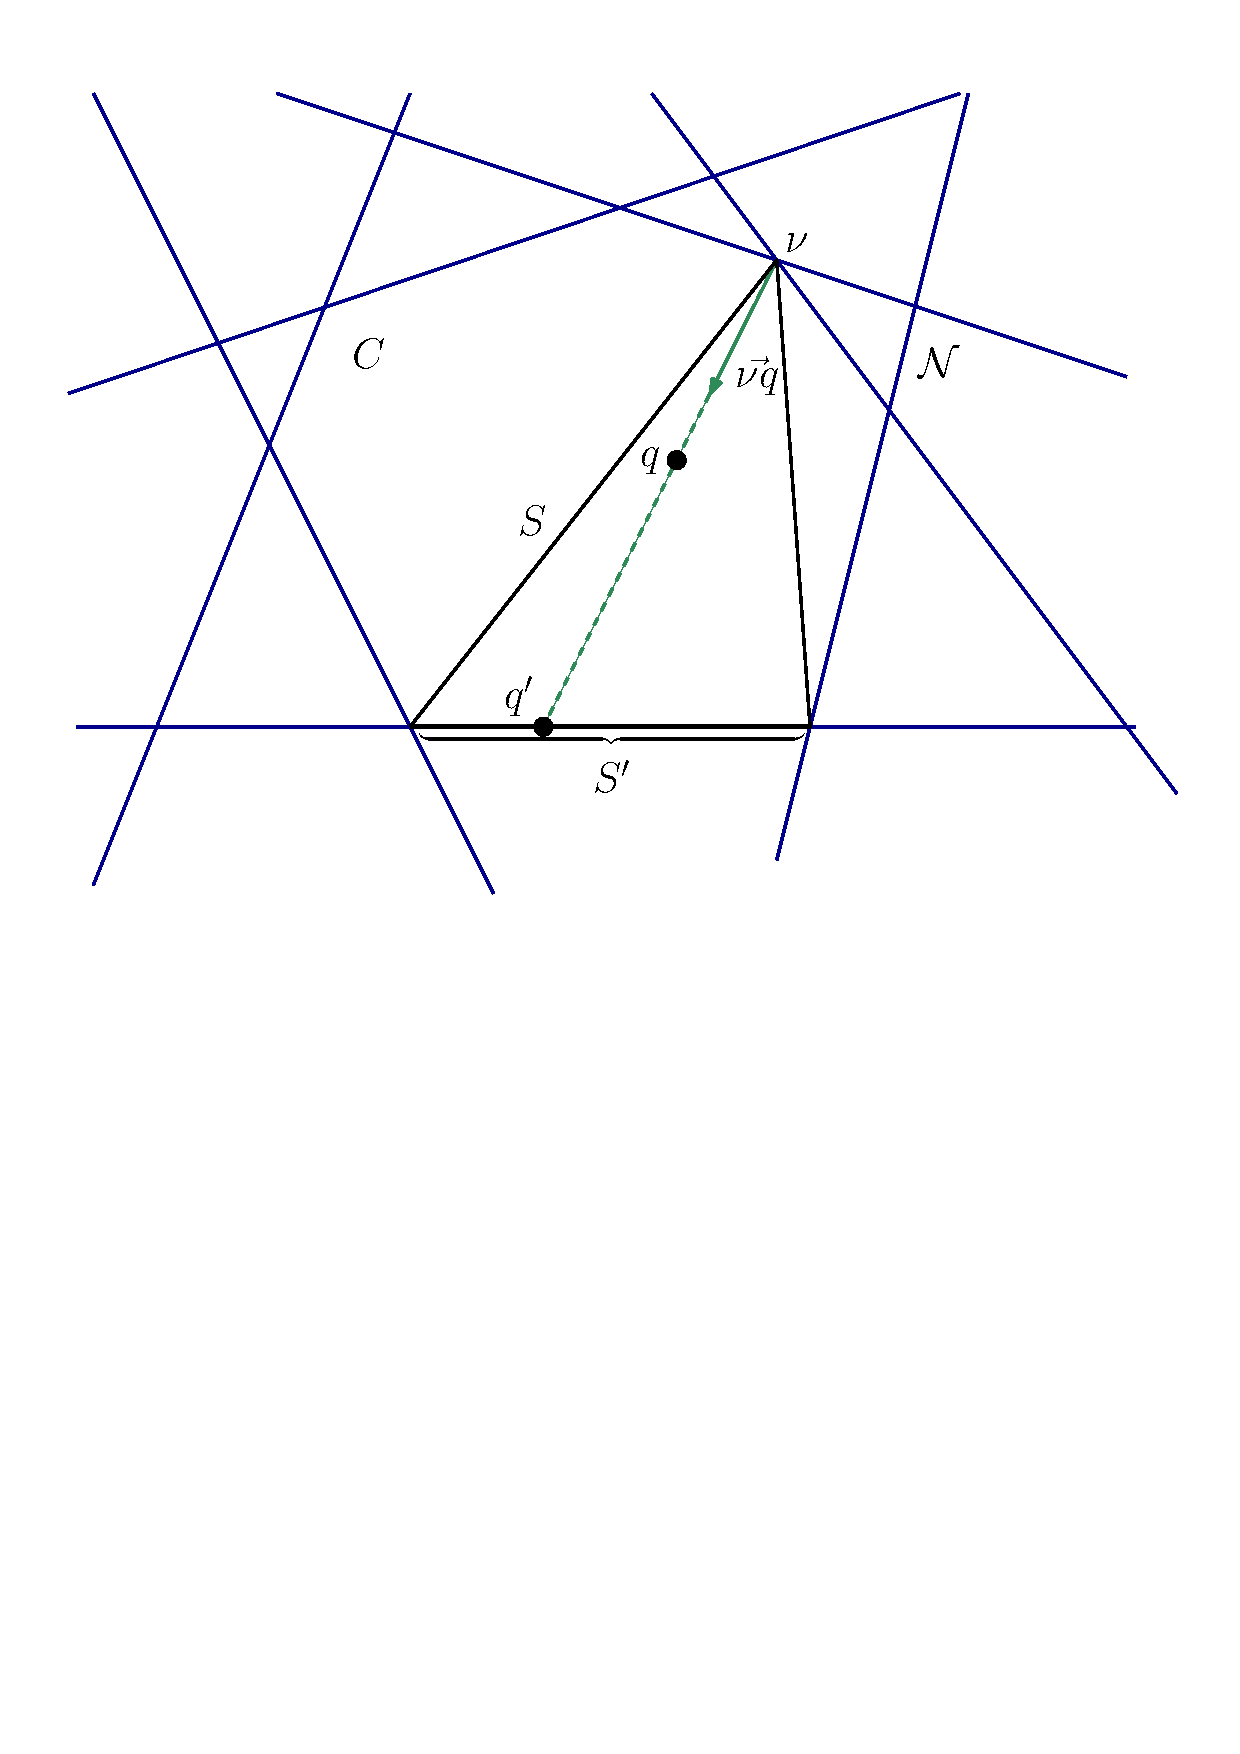
\includegraphics[trim=90 47 50 13,clip=true,height=0.25\textheight]{figures/simplex}
\caption{%
Illustration of a step of Algorithm~\ref{algo:simplex}.
}
\label{fig:meiser:step}
\end{center}
\end{figure}

\subsubsection{Assembling the pieces}

Let us summarize the algorithm
\begin{algorithm}\label{algo:meiser}
\item[input] \(q \in {[-1,1]}^n\)
\item[1.] Pick \(O(n^2 \log n)\) hyperplanes of $\Hy$ at random and locate $q$
in this arrangement. Call $\cell$ the cell containing $q$.
\item[2.] Construct the simplex \(\simplex\) containing \(q\) and inscribed in
\(\cell\), using Algorithm~\ref{algo:simplex}.
\item[3.] For every hyperplane of $\Hy$ containing $\simplex$, output a solution.
\item[4.] Recurse on hyperplanes of $\Hy$ intersecting the interior of $\simplex$.
\end{algorithm}

The query complexity of step \step{1} is $O(n^2 \log n)$, and that of step
\step{2} is $O(n^3 \log n)$. Steps \step{3} and \step{4} do not involve any
query at all. The recursion depth is $O(\log \card{\Hy})$, with $|\Hy|=O(n^k)$,
hence the total query complexity of this algorithm is $O(n^3 \log^2 n)$. This
proves the first part of Theorem~\ref{thm:cube}.\\

We can also consider the overall complexity of the algorithm in the RAM model,
that is, taking into account the steps that do not require any query, but for
which we still have to process the set $\Hy$. Note that the complexity
bottleneck of the algorithm are steps \step{3}-\step{4}, where we need to prune
the list of hyperplanes according to their relative positions with respect to
$\simplex$. For this purpose, we simply maintain explicitly the list of all
hyperplanes, starting with the initial set corresponding to all $k$-tuples.
Then the pruning step can be performed by looking at the position of each
vertex of $\simplex$ relative to each hyperplane of $\Hy$.
Because in our case hyperplanes have only $k$ nonzero coefficients, this uses a
number of integer arithmetic operations on $\tilde{O}(n)$ bits integers that is
proportional to the number of vertices times the number of hyperplanes.
(For the justification of the bound on the number of bits needed to represent
vertices of the arrangement see \S\ref{app:bound}.)
Since we recurse on a fraction of the set, the overall complexity is
$\tilde{O}(n^2\card{\Hy}) = \tilde{O}(n^{k+2})$. The next section is devoted
to improving this running time.



\subsection{Time complexity}
\label{paper:ksum-algorithm:contrib:time-complexity}

Proving the second part of Theorem~\ref{thm:cube} involves efficient implementations of
the two most time-consuming steps of Algorithm~\ref{algo:meiser}.
In order to efficiently implement the pruning
step, we define an intermediate problem, that we call the \emph{double $k$-SUM}
problem.
\begin{problem}[double $k$-SUM]
	Given two vectors $\nu_1, \nu_2 \in {[-1,1]}^n$, where the coordinates of
	$\nu_i$ can be written down as fractions whose numerator and denominator
	lie in the interval $[-M,M]$, enumerate all
	$i\in {[n]}^k$ such that
	$$
	\left(\sum_{j=1}^{k} \nu_{1,i_j}\right)
	\left(\sum_{j=1}^{k} \nu_{2,i_j}\right)
	< 0.
	$$
\end{problem}


In other words, we wish to list all hyperplanes of $\Hy$
intersecting the open line segment $\nu_1\nu_2$.
We give an efficient output-sensitive algorithm for this problem.

\begin{problem}[double $k$-SUM]
	Given two vectors $\nu_1, \nu_2 \in {[-1,1]}^n$, where the coordinates of
	$\nu_i$ can be written down as fractions whose numerator and denominator
	lie in the interval $[-M,M]$, enumerate all
	$i\in {[n]}^k$ such that
	$$
	\left(\sum_{j=1}^{k} \nu_{1,i_j}\right)
	\left(\sum_{j=1}^{k} \nu_{2,i_j}\right)
	< 0.
	$$
\end{problem}

\begin{proof}
	If $k$ is even, we consider all possible $\frac{k}{2}$-tuples of numbers in
	$\nu_1$ and $\nu_2$ and sort their sums in increasing order. This takes time
	$O(n^{\frac{k}{2}} \log n)$ and yields two permutations $\pi_1$ and $\pi_2$
	of $[n^\frac{k}{2}]$.
	If $k$ is odd, then we sort both the $\lceil\frac{k}{2}\rceil$-tuples and
	the $\lfloor\frac{k}{2}\rfloor$-tuples. For simplicity, we will only
	consider the even case in what follows. The odd case carries through.

	We let $N = n^\frac{k}{2}$. For $i \in [N]$ and $m \in \{1,2\}$, let
	$\Sigma_{m,i}$ be the sum of the $\frac{k}{2}$ components of the $i$th
	$\frac{k}{2}$-tuple in $\nu_m$, in the order prescribed by $\pi_m$.

	We now consider the two $N \times N$ matrices $M_1$ and $M_2$ giving all
	possible sums of two $\frac{k}{2}$-tuples, for both $\nu_1$ with the ordering
	$\pi_1$ and $\nu_2$ with the ordering $\pi_2$.

	We first solve the $k$-SUM problem on $\nu_1$, by finding the sign of all
	pairs $\Sigma_{1,i} + \Sigma_{1,j}$, $i, j \in [N]$. This can be done in
	time $O(N)$ by parsing the matrix $M_1$, just as in the standard \(k\)-SUM algorithm.
        We do the same with $M_2$.

	The set of all indices $i, j \in [N]$ such that $\Sigma_{1,i} +
	\Sigma_{1,j}$ is positive forms a staircase in $M_1$. We sweep $M_1$ column
	by column in order of increasing $j \in [N]$, in such a way that the number
	of indices $i$ such that $\Sigma_{1,i} + \Sigma_{1,j} > 0$ is growing.
	For each new such value $i$ that is encountered during the sweep, we insert
	the corresponding $i' = \pi_2(\pi_1^{-1}(i))$ in a balanced binary search
	tree.

	After each sweep step in $M_1$ --- that is, after incrementing $j$ and
	adding the set of new indices $i'$ in the tree --- we search the tree to
	identify all the indices $i'$ such that $\Sigma_{2,i'} + \Sigma_{2,j'} <
	0$, where $j' = \pi_2(\pi_1^{-1}(j))$. Since those indices form an interval
	in the ordering $\pi_2$ when restricted to the indices in the tree, we can
	search for the largest $i_0'$ such that $\Sigma_{2,i_0'} < -\Sigma_{2,j'}$
	and retain all indices $i' \le i_0'$ that are in the tree. If we denote by
	$z$ the number of such indices, this can be done in $O(\log N + z) = O(\log
	n + z)$ time. Now all the pairs $i', j'$ found in this way are such that
	$\Sigma_{1,i} + \Sigma_{1,j}$ is positive and $\Sigma_{2,i'} +
	\Sigma_{2,j'}$ is negative, hence we can output the corresponding
	$k$-tuples. To get all the pairs $i', j'$ such that
	$\Sigma_{1,i} + \Sigma_{1,j}$ is negative and $\Sigma_{2,i'} +
	\Sigma_{2,j'}$ positive, we repeat the sweeping algorithm after swapping the
	roles of $\nu_1$ and $\nu_2$.

	Every matching $k$-tuple is output exactly once, and every
	$\frac{k}{2}$-tuple is inserted at most once in the binary search tree.
	Hence the algorithm runs in the claimed time.

	Note that we only manipulate rational numbers that are the sum of at most
	$k$ rational numbers of size $O(\log M)$.
\end{proof}

Now observe that a hyperplane intersects the interior of a simplex if and only
if it intersects the interior of one of its edges. Hence given a simplex
$\simplex$ we can find all hyperplanes of $\Hy$ intersecting its interior by
running the above algorithm ${n\choose 2}$ times, once for each pair of
vertices $(\nu_1,\nu_2)$ of $\simplex$, and take the union of the solutions.
The overall running time for this implementation will therefore be
$\tilde{O}(n^2 (n^{\lceil \frac k2 \rceil} \log M + Z))$, where $Z$ is at most the
number of intersecting hyperplanes and $M$ is to be determined later.
This provides an implementation of the pruning step in Meiser's algorithm, that
is, step~\step{4} of Algorithm~\ref{algo:meiser}.

\begin{corollary}\label{cor:double}
	Given a simplex $\simplex$, we can compute all $k$-SUM hyperplanes
	intersecting its interior in $\tilde{O}(n^2 (n^{\lceil \frac k2 \rceil}
	\log M + Z))$ time, where $\log M$ is proportional to the number of bits
	necessary to represent $\simplex$.
\end{corollary}

In order to detect solutions in step~\step{3} of Algorithm~\ref{algo:meiser}, we also
need to be able to quickly solve the following problem.
\begin{problem}[multiple $k$-SUM]
	Given $d$ points $\nu_1,\nu_2,\ldots,\nu_d \in \R^n$, where the coordinates of
	$\nu_i$ can be written down as fractions whose numerator and denominator
	lie in the interval $[-M,M]$,
	decide whether there exists a hyperplane with equation of the form $x_{i_1}
	+ x_{i_2} + \cdots + x_{i_k} = 0$ containing all of them.
\end{problem}

Here the standard $k$-SUM algorithm can be applied, taking advantage of
the fact that the coordinates lie in a small discrete set.
\begin{lemma}\label{lem:ksum}
	$k$-SUM on $n$ integers $\in [-V,V]$ can be solved in time
	$\tilde{O}(n^{\ckt}\log V)$.
\end{lemma}

\begin{lemma}\label{lem:multiple}
	Multiple $k$-SUM can be solved in time $\tilde{O}(dn^{\ckt+2}\log M)$.
\end{lemma}
\begin{proof}
	Let $\mu_{i,j}$ and $\delta_{i,j}$ be the numerator and denominator of
	$\nu_{i,j}$ when written as an irreducible fraction. We define
	$$
		\zeta_{i,j} = \nu_{i,j}\prod_{\mathclap{(i,j) \in [d]\times[n]}} \delta_{i,j} =
		\frac{\mu_{i,j}\displaystyle\prod_{\mathclap{(i',j') \in [d]\times[n]}} \delta_{i',j'}}{\delta_{i,j}}.
	$$
	By definition $\zeta_{i,j}$ is an integer and its absolute value is bounded
	by $U = M^{n^2}$, that is, it can be
	represented using $O(n^2 \log M)$ bits. Moreover, if one of the hyperplanes
	contains the point $(\zeta_{i,1},\zeta_{i,2},\ldots,\zeta_{i,n})$, then it
	contains $\nu_i$. Construct $n$ integers of $O(dn^2 \log M)$ bits that can
	be written $\zeta_{1,j}+U,\zeta_{2,j}+U,\ldots,\zeta_{d,j}+U$ in base
	$2Uk+1$. The answer to our decision problem is ``yes'' if and only if there
	exists $k$ of those numbers whose sum is $kU,kU,\ldots,kU$. We simply
	subtract the number $U,U,\ldots,U$ to all $n$
	input numbers to obtain a standard $k$-SUM instance on $n$ integers of
	$O(dn^2 \log M)$ bits.
\end{proof}

We now have efficient implementations of steps \step{3} and \step{4}
of Algorithm~\ref{algo:meiser} and can proceed to the proof of the second part
of Theorem~\ref{thm:cube}.

\begin{proof}
The main idea consists in modifying the first iteration of Algorithm~\ref{algo:meiser}, by
letting $\varepsilon = \Theta(n^{-\frac{k}{2}})$.
Hence we pick a random subset $\net$ of
$O(n^{k/2 + 2} \log n)$ hyperplanes in $\Hy$ and use this as an \enet.
This can be done efficiently, as shown in~\S\ref{app:sampling}.

Next, we need to locate the input $q$ in the arrangement induced by
$\net$. This can be done by running Algorithm~\ref{algo:meiser} on the set
$\net$. From the previous considerations on Algorithm~\ref{algo:meiser}, the
running time of this step is
$$
O(n|\net|) = \tilde{O}(n^{k/2 + 4}),
$$
and the number of queries is $O(n^3\log^2 n)$.

Then, in order to prune the hyperplanes in $\Hy$, we have to
compute a simplex $\simplex$ that does not intersect any hyperplane of
$\net$. For this, we observe that the above call to Algorithm~\ref{algo:meiser}
involves computing a sequence of simplices for the successive pruning
steps. We save the description of those simplices. Recall that there are
$O(\log n)$ of them, all of them contain the input $q$ and have vertices
coinciding with vertices of the original arrangement $\arrangement(\Hy)$. In
order to compute a simplex $\simplex$ avoiding all hyperplanes of
$\net$, we can simply apply Algorithm~\ref{algo:simplex} on the set of
hyperplanes bounding the intersection of these simplices. The running time
and number of queries for this step are bounded respectively by
$n^{O(1)}$ and $O(n^2\log n)$.

Note that the vertices of $\simplex$ are not vertices
of $\arrangement(\Hy)$ anymore. However, their coordinates lie in a finite set
(see~\S\ref{app:bound})
\begin{lemma}\label{lem:bound}
Vertices of $\simplex$ have rational coordinates whose fraction representations
have their numerators and denominators absolute values bounded above by
$C^{4n^5} n^{2n^5+n^3+\frac n2}$, where $C$ is a constant.
\end{lemma}

We now are in position to perform the pruning of the hyperplanes in $\Hy$ with
respect to $\simplex$. The number of remaining hyperplanes after the pruning is
at most $\varepsilon n^k = O(n^{k/2})$. Hence from Corollary~\ref{cor:double}, the
pruning can be performed in time proportional to $\tilde{O}(n^{\ceil{k/2} + 7})$.

Similarly, we can detect any hyperplane of $\Hy$ containing $\simplex$ using the
result of Lemma~\ref{lem:multiple} in time $\tilde{O}(n^{\lceil k/2\rceil +
8})$. Note that those last two steps do not require any query.

Finally, it remains to detect any solution that may lie in the remaining
set of hyperplanes of size $O(n^{k/2})$. We can again fall back
on Algorithm~\ref{algo:meiser}, restricted to those hyperplanes. The running
time is $\tilde{O}(n^{k/2 + 2})$, and the number of queries is still
$O(n^3 \log^2 n)$.

Overall, the maximum running time of a step is $\tilde{O}(n^{\ceil{\frac{k}{2}} + 8})$,
while the number of queries is always bounded by $O(n^3\log^2 n)$.

\end{proof}


\subsection{Query size}
\label{paper:ksum-algorithm:contrib:query-size}

In this section, we consider a simple blocking scheme that allows us to explore
a tradeoff between the number of queries and the size of the queries.

\begin{lemma}
\label{lem:block}
For any integer $b>0$, an instance of the \(k\)-SUM problem on $n>b$ numbers can be split into
$O(b^{k-1})$ instances on at most $k\lceil \frac{n}{b}\rceil$ numbers, so that every $k$-tuple
forming a solution is found in exactly one of the subproblems.
The transformation can be carried out in time $O(n\log n + b^{k-1})$.
\end{lemma}
\begin{proof}
Given an instance on $n$ numbers, we can sort them in time $O(n\log n)$, then partition
the sorted sequence into \(b\) consecutive blocks \(B_1, B_2,\ldots ,B_b\) of equal size.
This partition can be associated with a partition of the real line
into $b$ intervals, say $I_1, I_2,\ldots ,I_b$. Now consider the partition of $\R^k$
into grid cells defined by the $k$th power of the partition $I_1, I_2,\ldots ,I_b$. The
hyperplane of equation $x_1 + x_2 +\cdots +x_k = 0$ hits $O(b^{k-1})$ such grid cells.
Each grid cell $I_{i_1}\times I_{i_2}\times \cdots \times I_{i_k}$ corresponds to a
\(k\)-SUM problem on the numbers in the set $B_{i_1}\cup B_{i_2}\cup \ldots \cup B_{i_k}$ (note that
the indices $i_j$ need not be distinct). Hence each such instance has size at most $k\lceil \frac{n}{b}\rceil$.
\end{proof}

Combining Lemma~\ref{lem:block} and Theorem~\ref{thm:cube} directly yields our
second contribution.
%
\TheoremKSUMQuerySize*

The following two corollaries are obtained by taking
$b=\Theta(\polylog(n))$, and $b=\Theta(n^{\alpha})$, respectively
\begin{corollary}\label{cor:logn}
There exists an $o(n)$-linear decision tree of
depth $\tilde{O}(n^3)$ solving the \(k\)-SUM problem.
Moreover, this decision tree can be implemented as an
$\tilde{O}(n^{\ceil{\frac{k}{2}}+8})$ Las Vegas algorithm.
\end{corollary}
\begin{corollary}\label{cor:ne}
For any $\alpha$ such that $0<\alpha<1$,
there exists an $O(n^{1-\alpha})$-linear decision tree of
depth $\tilde{O} (n^{3+(k-4)\alpha})$ solving the \(k\)-SUM problem.
Moreover, this decision tree can be implemented as an
$\tilde{O}(n^{(1+\alpha)\frac{k}{2} + 8.5})$
Las Vegas algorithm.
\end{corollary}

Note that the latter query complexity improves on $\tilde{O}(n^{\frac{k}{2}})$
whenever \(\alpha < \frac{k-6}{2k-8}\) and $k\ge 7$.
By choosing $\alpha=\frac{k-6}{2k-8}-\frac{\beta}{k-4}$
we obtain $O(n^{1-\frac{k-6}{2k-8}+\frac{\beta}{k-4}})$-linear decision trees
of depth
$\tilde{O}(n^{\frac k2 - \beta})$
for any $k \ge 7$.
Hence for instance, we obtain
$O(n^{\frac{3}{4}+\frac{\beta}{4}})$-linear decision trees of depth
$\tilde{O}(n^{4-\beta})$ for the \dsum[8] problem.



\section{Missing Details}\label{paper:ksum-algorithm:details}

This section regroups the missing details of the algorithms described in the
previous one (\S\ref{paper:ksum-algorithm:proofs}).

In \S\ref{app:keeplinear} we show how to keep the queries linear even though it
is not evident at first sight that they are because of all the algebra
generated by the recursive steps of the simplex construction.
%
In \S\ref{app:act} we show that our linear decision tree can be implemented in
the same time on the algebraic computation tree model, even though some linear
queries may involve all members of the input, and hence have superconstant
cost.
%
In \S\ref{app:sampling} we explain how to efficiently implement uniform random sampling
for the construction of large \(\varepsilon\)-nets.
%
In \S\ref{app:bound} we bound the size of the numbers manipulated by the
word-RAM implementation of our \(k\)-SUM algorithm.

\subsection{Keeping queries linear in Algorithm~\ref*{algo:simplex}}
\label{app:keeplinear}
In Algorithm~\ref{algo:simplex}, we want to ensure that the queries we make in step
\step{2} are linear and that the queries we will make in the recursion step
remain linear too.
\begin{lemma}
	Algorithm~\ref{algo:simplex} can be implemented so that it uses $O(n\card{I})$ linear queries.
\end{lemma}%
\begin{proof}
Let us first analyze what the queries of step \step{2} look like. In addition
to the input point \(q\) we are given a vertex \(\nu\) and we want to find the
projection \(q'\) of \(q\) in direction \(\vec{\nu q}\) on the hyperplanes of
\(\I_{\theta}\). Let the equation of \(H_{i}\) be \(\Pi_{i}(x) =
c_{i} + d_{i}
\cdot x = 0\) where \(c_{i}\) is a scalar and \(d_{i}\) is a
vector.
The projection of \(q\) along \(\vec{\nu q}\) on a hyperplane \(H_i\) can thus
be written\footnote{Note that we project from \(\nu\) instead of \(q\). We are
allowed to do this since \(\nu + \lambda_{i} \vec{\nu q} = q + (\lambda_i - 1)
\vec{\nu q}\) and there is no hyperplane
separating \(q\) from \(\nu\).}
\(\rho(q,\nu,H_i) = \nu + \lambda_{i} \vec{\nu q}\) such that \(\Pi_{i}(\nu +
		\lambda_{i} \vec{\nu q}) = c_{i} + d_{i} \cdot \nu +
		\lambda_{i} d_{i} \cdot
\vec{\nu q} = 0\). Computing the closest hyperplane amounts to finding
\(\lambda_{\theta} = \min_{\lambda_i > 0} \lambda_i\). Since \(\lambda_i = -
\frac{c_i + d_i \cdot \nu}{d_i \cdot \vec{\nu q}}\) we can test whether
\(\lambda_i > 0\)
using the linear query\footnote{Note that if $c_i + d_i \cdot \nu = 0$ then
$\lambda_i=0$, we can check this beforehand for free.}
\(-\frac{d_i \cdot \vec{\nu q}}{c_i + d_i
\cdot \nu} \ask{>} 0\). Moreover, if \(\lambda_i > 0\) and \(\lambda_j > 0\)
we can test whether $\lambda_i < \lambda_j$ using the linear query \(
\frac{d_i \cdot \vec{\nu q}}{c_i + d_i \cdot \nu}
\ask{<}
\frac{d_j \cdot \vec{\nu q}}{c_j + d_j \cdot \nu}\).
Step \step{2} can thus be achieved using \(O(1)\) \((2k)\)-linear queries per
hyperplane of \(\net\).

In step \step{4}, the
recursive step is carried out on \(q' = \nu + \lambda_{\theta} \vec{\nu q} = \nu -
\frac{c_{\theta} + d_{\theta} \cdot \nu}{d_{\theta} \cdot \vec{\nu q}}
\vec{\nu q}\) hence comparing \(\lambda'_i\) to \(0\) amounts to performing the
query \(-\frac{d_i \cdot \vec{\nu q}'}{c_i + d_i \cdot \nu'}
\ask{>} 0\), which is not linear in \(q\). The same goes for comparing
\(\lambda'_i\) to \(\lambda'_j\) with the query
\(\frac{d_i \cdot \vec{\nu q}'}{c_i + d_i \cdot \nu'}
\ask{<}
\frac{d_j \cdot \vec{\nu q}'}{c_j + d_j \cdot \nu'}\).

However, we can multiply both sides of the inequality test by \(d_\theta
\vec{\nu q}\) to keep the queries linear as shown below. We must be careful to
take into account the sign of the expression \(d_\theta \vec{\nu q}\), this
costs us one additional linear query.

This trick can be used at each step of the recursion. Let \(q^{(0)} = q\),
then we have
$$
	q^{(s+1)} = \nu^{(s)} - \frac{c_{\theta_{s}} + d_{\theta_{s}} \cdot
	\nu^{(s)}}{d_{\theta_{s}} \cdot \vec{\nu q}^{(s)}}\vec{\nu q}^{(s)}
$$
and \( (d_{\theta_{s}}\cdot \vec{\nu q}^{(s)}) q^{(s+1)}\) yields a vector
whose components are linear in \(q^{(s)}\).
Hence,
\( (\prod_{k=0}^{s} d_{\theta_{k}} \cdot \vec{\nu q}^{(k)})
 q^{(s+1)}\) yields a vector
whose components are linear in \(q\),
and for all pairs of vectors \(d_i\) and \(\nu^{(s+1)}\)
we have that \( (\prod_{k=0}^{s} d_{\theta_{k}} \cdot \vec{\nu q}^{(k)}) (d_i
\cdot \vec{\nu q}^{(s+1)})\) is linear in \(q\).

Hence at the $s$th recursive step of the algorithm, we will perform
at most \(\card{\net}\) linear queries of the type
$$
	-\left(\prod_{k=0}^{s-1} d_{\theta_{k}} \cdot \vec{\nu q}^{(k)}\right)
\frac{d_i \cdot \vec{\nu q}^{(s)}}{c_i + d_i \cdot
	\nu^{(s)}} \ask{>} 0
$$
\(\card{\net} - 1\) linear queries of the type
$$
	\left(\prod_{k=0}^{s-1} d_{\theta_{k}} \cdot \vec{\nu q}^{(k)}\right)
	\frac{d_i \cdot \vec{\nu q}^{(s)}}{c_i + d_i \cdot \nu^{(s)}}
\ask{<}
\left(\prod_{k=0}^{s-1} d_{\theta_{k}} \cdot \vec{\nu q}^{(k)}\right)
\frac{d_j \cdot \vec{\nu q}^{(s)}}{c_j + d_j \cdot \nu^{(s)}}
$$
and a single linear query of the type
$$
	d_{\theta_{s-1}} \cdot \vec{\nu q}^{(s-1)} \ask{<} 0.
$$

In order to detect all hyperplanes \(H_i\) such that \(\lambda_i =
\lambda_\theta\) we can afford to compute the query $f(q) > g(q)$ for all query
$f(q) < g(q)$ that we issue, and vice versa.

Note that, without further analysis, the queries can become \(n\)-linear as
soon as we enter the \(\frac{n}{k}^{\text{th}}\) recursive step.
\end{proof}


\subsection{Algebraic Computation Trees}%
\label{app:act}

The following theorem follows immediately from
the analysis of the linearity of queries
\begin{theorem}\label{thm:act}
	The algebraic computation tree complexity of \(k\)-LDT is
	\(\tilde{O}(n^3)\).
\end{theorem}

\begin{proof}
We go through each step of Algorithm~\ref{algo:meiser}.
Indeed, each \(k\)-linear query of step \step{1} can be implemented as
\(O(k)\) arithmetic operations, so step \step{1} has complexity
\(O(\card{\net})\).
The construction of the simplex in step \step{2} must be handled carefully.
What we need to show is that each \(n\)-linear query we use can be implemented
using $O(k)$ arithmetic operations. It is not difficult to see from the
expressions given in~\S\ref{app:keeplinear} that a constant number of arithmetic
operations and dot products suffice to
compute the queries. A dot product in this case involves a constant number
of arithmetic operations because the \(d_i\) are such that they each have
exactly \(k\) non-zero components. The only expression that involves a
non-constant number of operations is the product \(\prod_{k=0}^{s}
d_{\theta_{k}} \cdot \vec{\nu q}^{(k)}\), but this is equivalent to
\((\prod_{k=0}^{s-1}
	d_{\theta_{k}} \cdot \vec{\nu q}^{(k)})(d_{\theta_{s}} \cdot
	\vec{\nu q}^{(s)})\)
where the first factor has already been computed during a previous step and
the second factor is of constant complexity. Since each query costs a constant
number of arithmetic operations and branching operations, step \step{2}
has complexity \(O(n\card{\net})\).
Finally, steps \step{3} and \step{4} are free since they do not involve the
input. The complexity of Algorithm~\ref{algo:meiser} in this model is thus also \(O(n^3
\log n \log \card{\Hy})\).
\end{proof}



\subsection{Uniform random sampling}
\label{app:sampling}

Theorem~\ref{thm:enet} requires us to pick a sample of the hyperplanes
uniformly at random. Actually the theorem is a little stronger; we can draw
each element of $\net$ uniformly at random, only keeping distinct elements.
This is not too difficult to achieve for $k$-LDT when the $\alpha_i,i\in[k]$
are all distinct: to pick a hyperplane of the form $\alpha_0 + \alpha_1 x_{i_1}
+ \alpha_2 x_{i_2} + \cdots + \alpha_k x_{i_k} = 0$ uniformly at random, we can
draw each $i_j\in[n]$ independently and there are $n^k$ possible outcomes.
However, in the case of $k$-SUM, we only have $\binom{n}{k}$ distinct
hyperplanes. A simple dynamic programming approach solves the problem for
\(k\)-SUM. For \(k\)-LDT we can use the same approach, once for each class of equal
$\alpha_i$.

\begin{lemma}
	Given $n\in\N$ and $(\alpha_0,\alpha_1,\ldots,\alpha_k) \in \R^{k+1}$,
	$m$ independent uniform random draws of
	hyperplanes in $\R^n$ with equations of the form
	$\alpha_0 + \alpha_1 x_{i_1} + \alpha_2 x_{i_2} + \cdots + \alpha_k x_{i_k} = 0$
	can be computed in time $O(mk^2 \log n)$
	and preprocessing time $O(k^2 n)$.
\end{lemma}
\begin{proof}
	We want to pick
	an assignment
	$a=\enum{(\alpha_1,x_{i_1}),(\alpha_2,x_{i_2}),\ldots,(\alpha_k,x_{i_k})}$
	uniformly at random. Note that all $x_i$ are distinct while the $\alpha_j$
	can be equal.

	Without loss of generality, suppose $\alpha_1 \le \alpha_2 \le \cdots \le
	\alpha_k$. There is a bijection between assignments and lexicographically
	sorted $k$-tuples
	$((\alpha_1,x_{i_1}),(\alpha_2,x_{i_2}),\ldots,(\alpha_k,x_{i_k}))$.

	Observe that $x_{i_j}$ can be drawn independently of $x_{i_{j'}}$ whenever
	$\alpha_j \neq \alpha_{j'}$. Hence, it suffices to generate a lexicographically sorted
	$\card{\chi}$-tuple of $x_i$ for each class $\chi$ of equal $\alpha_i$.

	Let $\omega(m,l)$ denote the number of lexicographically sorted $l$-tuples,
	where each element comes from a set of $m$ distinct $x_i$.
	We have
	$$
		\omega(m,l) = \begin{cases}
			1 & \text{if}\ l = 0\\
			\sum_{i=1}^{m}\omega(i,l-1) & \text{otherwise.}
		\end{cases}
	$$

	To pick such a tuple $(x_{i_1},x_{i_2},\ldots,x_{i_l})$ uniformly at random
	we choose $x_{i_l} = x_o$ with probability
	$$
		P(x_{i_l} = x_o) = \begin{cases}
			0 & \text{if}\ o > m\\
			\frac{\omega(o,l-1)}{\omega(m,l)} & \text{otherwise}
		\end{cases}
	$$
	that we append to a prefix $(l-1)$-tuple (apply the procedure recursively),
	whose elements come from a set of $o$ symbols. If $l=0$ we just
	return the empty tuple.

	Obviously, the probability for a given $l$-tuple to be picked is equal to
	$\frac{1}{\omega(m,l)}$.

	Let $X$ denote the partiton of the $\alpha_i$ into equivalence classes,
	then the number of
	assignments is equal to $\prod_{\chi \in X}\omega(n,\card{\chi})$.
	(Note that for $k$-SUM this is simply $\omega(n,k)$ since there is only a
	single class of equivalence.)
	For each equivalence class $\chi$ we draw independently a lexicographically
	sorted $\card{\chi}$-tuple on $n$ symbols using the procedure
	above. This yields a given assignment with probability
	$\frac{1}{\prod_{\chi \in X}\omega(n,\card{\chi})}$.
	Hence, this corresponds to a uniform random draw over the assignments.

	It is a well known fact that $\omega(n,k)=\binom{n+k-1}{k-1}$, hence each
	number we manipulate fits in $O(k \log n)$ bits, that is, $O(k)$ words.
	Moreover $\omega(n,k) = \omega(n-1,k) + \omega(n-1,k-1)$ so each
	$\omega(m,l)$ can be computed using a single addition on numbers of $O(k)$
	words.

	For given $n$ and $k$, there are at most $nk$ values $\omega(m,l)$ to
	compute, and for a given $k$-LDT instance, it must be computed only once.
	One way to perform the random draws is to compute the cumulative
	distribution functions of the discrete distributions defined above, then to
	draw $x_{i_l}$, we use binary search to find a generated random integer of
	$O(k)$ words in the cumulative distribution function. Computing the
	values $\omega(m,l)$ and all cumulative distributions functions can be done
	as a preprocessing step in $O(k^2 n)$ time. Assuming the generation
	of a random sequence of words takes linear time, performing a random draw
	takes time $O(k^2 \log n)$.

\end{proof}


\subsection{Proof of Lemma~\ref*{lem:bound}}
\label{app:bound}

\begin{theorem}[Cramer's rule]\label{thm:cramer}
	If a system of $n$ linear equations for $n$ unknowns, represented in matrix
	multiplication form $Ax=b$,
	has a unique solution $x=(x_1,x_2,\ldots,x_n)^T$ then, for all $i \in [n]$,
	$$
		x_i = \frac{\det(A_i)}{\det(A)}
	$$
	where $A_i$ is $A$ with the $i$th column replaced by the column vector $b$.
\end{theorem}


\begin{lemma}[Meyer auf der Heide\cite{M84}]\label{lem:detZ}
	The absolute value of the determinant of an $n\times n$ matrix $M =
	M_{i=1\ldots n,j=1\ldots n}$ with integer entries is an integer that is at
	most $C^n n^{\frac n2}$, where $C$ is the maximum absolute value in $M$.
\end{lemma}
\begin{proof}
	The determinant of $M$ must be an integer
	and is the volume of the
	hyperparalleliped spanned by the row vectors of $M$, hence
	$$
	|\det(M)| \le \prod_{i=1}^n \sqrt{\sum_{j=1}^{n} M_{i,j}^2} \le {(\sqrt{n C^2})}^{n} \le C^n n^\frac n2.
	$$
\end{proof}

\begin{lemma}\label{lem:detQ}
	The determinant of an $n\times n$ matrix $M = M_{i=1\ldots n,j=1\ldots n}$ with
	rational entries can be represented as a fraction whose numerators and
	denominators absolute values are bounded above by
	${(ND^{n-1})}^n n^{\frac n2}$ and $D^{n^2}$
	respectively, where $N$ and $D$
	are respectively the maximum absolute value of a numerator and a
	denominator in $M$.
\end{lemma}
\begin{proof}
	Le $\delta_{i,j}$ denote the denominator of $M_{i,j}$.
	Multiply each row $M_i$ of $M$ by $\prod_j \delta_{i,j}$.
	Apply Lemma~\ref{lem:detZ}.
\end{proof}

We can now proceed to the proof of Lemma~\ref{lem:bound}.
\begin{proof}
	Coefficients of the hyperplanes of the arrangement are constant rational
	numbers, those can be changed to constant integers (because each
	hyperplane has at most $k$ nonzero coefficients). Let $C$ denote the
	maximum absolute value of those coefficients.

	Because of Theorem~\ref{thm:cramer} and Lemma~\ref{lem:detZ}, vertices of
	the arrangement have rational coordinates whose numerators and
	denominators absolute values are bounded above by $C^n n^{\frac n2}$.

	Given simplices whose vertices are vertices of the arrangement, hyperplanes
	that define the faces of those simplices have rational coefficients whose
	numerators and denominators absolute values are bounded above by $C^{2n^3}
	n^{n^3+\frac n2}$ by Theorem~\ref{thm:cramer} and Lemma~\ref{lem:detQ}.
	(Note that some simplices might be not fully dimensional, but we can handle
	those by adding vertices with coordinates that are not much larger than
	that of already existing vertices).

	By applying Theorem~\ref{thm:cramer} and Lemma~\ref{lem:detQ} again, we
	obtain that vertices of the arrangement of those new hyperplanes (and thus
	vertices of $\simplex$) have rational coefficients whose numerators and
	denominators absolute values are bounded above by $C^{4n^5} n^{2n^5+n^3+\frac n2}$.
\end{proof}

